\nchapter{Letters and Sounds}


\section{Sound System}
\noindent The Na'vi language has 20 consonant sounds, 7 vowel sounds
and two syllabic resonants Frommer calls ``pseudovowels.''
\LanguageLog

\subsection{Consonants}
Below are the consonants of Na'vi.  Phonemes in parentheses are Reef
Na'vi pronunciations of certain phonemes and assimilations, but which
don't get a separate spelling.

\begin{center}
\begin{tabular}{llllll}
 & Labial & Alveolar & Palatal & Velar & Glottal \\
Ejectives &	\N{px} [p'] & \N{tx} [t'] & & \N{kx} [k'] \\
Voiceless Stops & \N{p} [p] & \N{t} [t] & & \N{k} [k] & \N{’} [ʔ] \\
Voiced Stops    &  ([b])    & ([d])    &  & ([g]) \\
Affricate &             & \N{ts}  [ts] & ([tʃ]) \\
Voiceless fricatives & \N{f} [f] & \N{s} [s] & ([ʃ]) & & \N{h} [h] \\
Voiced fricatives & \N{v} [v] & \N{z} [z] \\
Nasals &         \N{m} [m] & \N{n} [n] & & \N{ng} [ŋ] \\
Liquids &         &  \N{r} [ɾ], \N{l} [l] \\
Glides &       \N{w} [w] & &  \N{y} [j] \\
\end{tabular}
\end{center}

\subsubsection{} The voiceless stops are unaspirated at the beginning
and middle of a word and un\-re\-lea\-sed at the end.  However, within a
phrase a final stop coming before a vowel will in natural speech be
released as the words flow together, \N{oel se\uwave{t o}mum}.
Unreleased stops will be most noticeable at major pauses, as in \N{oel
omum se\uwave{t}.}

\subsubsection{} The \N{r} is an alveolar flap.  The \N{l} is clear
and front, as in ``leaf,'' not the velarized, ``dark-l'' of English
``call''.

\subsubsection{} Frommer devised a scientific orthography in which two
of the digraphs were written as a single letter, \N{c} for \N{ts} and
\N{g} for \N{ng}.  The digraph system was easier for the actors, but
it has been also used by Frommer in media interviews and in most of
his own email.  The scientific orthography is only seen in a few early
emails to and from Frommer.  \label{l-and-s:cg}

\subsubsection{} Because plain stops can be used as syllable codas,
the more common ejective notation, \N{p'}, is too ambiguous:
\N{tsap'alute} is not *\N{tsapxalute}.
\LNWiki{21/12/2009}{https://wiki.learnnavi.org/index.php/Canon\%23Extracts_from_various_emails}

\newpage
\subsection{Vowels}
The vowel in parentheses only shows up as a distinct phoneme in Reef
Na'vi.  All the others are in both dialects.

\begin{center}
\begin{tabular}{ccccc}
\N{i} [i], \N{ì} [{\footnotesize I}]  & & & & (\N{ù} [ʊ]), \N{u} [u],[ʊ] \\
 & \N{e} [ɛ] & & & \N{o} [o] \\
 & & \N{ä} [æ] &  \N{a} [a] \\
\end{tabular}
\end{center}

\subsubsection{} Reef Na'vi pronounces \N{u} as [u] in all positions,
and \N{ù} as [ʊ] in all positions. \index{Reef Na'vi!ù@\textbf{ù}}
\LNWiki{8/1/2023}{http://naviteri.org/2023/01/reef-navi-part-1-phonetics-and-phonology/}

\subsubsection{} Forest Na'vi has merged the vowels \N{u} and \N{ù},
so that they are always [u] in open syllables, and may be either [u]
or [ʊ] in closed syllables.  \N{Lu} is always pronounced [lu],
while \N{pum} may be either [pum] or [pʊm].
\LNWiki{20/5/2010}{https://wiki.learnnavi.org/index.php/Canon/2010/March-June\%23The_Dual_sounds_of_.22u.22}

% 2023jan10 - don't do this for now.
%In this grammar words that are known to have \N{ù} in them in Reef
%Na'vi are spelled as such, such as \N{pùm}.  When using Forest Na'vi,
%simply treat these words as though spelled \N{pum}.

\subsubsection{} The diphthongs are \N{aw}, \N{ay}, \N{ew} and \N{ey}.
Only in diphthongs will \N{w} or \N{y} be seen at the end of a
syllable (\N{new}) or before a final consonant (\N{hawng}).  Syllable
shapes like \N{*niw} or \N{*hoyng} cannot occur.

\subsection{Pseudovowels} The pseudovowel \N{rr} is a syllabic,
trilled [r̩ː], and \N{ll} is a syllabic [l̩ː].

\subsection{Syllable Structure}
 Na'vi has a strict but straightforward syllable structure.

\begin{itemize*}
  \item A syllable is permitted to have no onset consonant (i.e., it
    may start with a vowel).
  \item A syllable is permitted to have no coda consonant (i.e., it
    may end with a vowel).
  \item Any consonant may start a syllable.
  \item A consonant cluster of \N{f s ts} $+$ \N{p, t, k, px, tx, kx,
    m, n, ng, r, l, w, y} may start a syllable (e.g., \N{tslam}, \N{ftu}).
  \item \N{P t k px tx kx ' m n l r ng} may occur in syllable-final position.
  \item \N{Ts f s h v z w y} may \textit{not} occur in syllable-final position.
  \item There are no consonant clusters in syllable-final position.
  \item \label{l-and-s:pseudo-no-null} A syllable with a pseudovowel
    must start with a consonant or consonant cluster and must not have
    a final consonant; this plays a role in lenition
    (\horenref{l-and-s:lenition:pseudovowel}) and the declension of nouns
    (\horenref{morph:decl:pseudovowel}).
\end{itemize*}

\noindent A visual representation of these core syllable structure rules:

\begin{center}\footnotesize
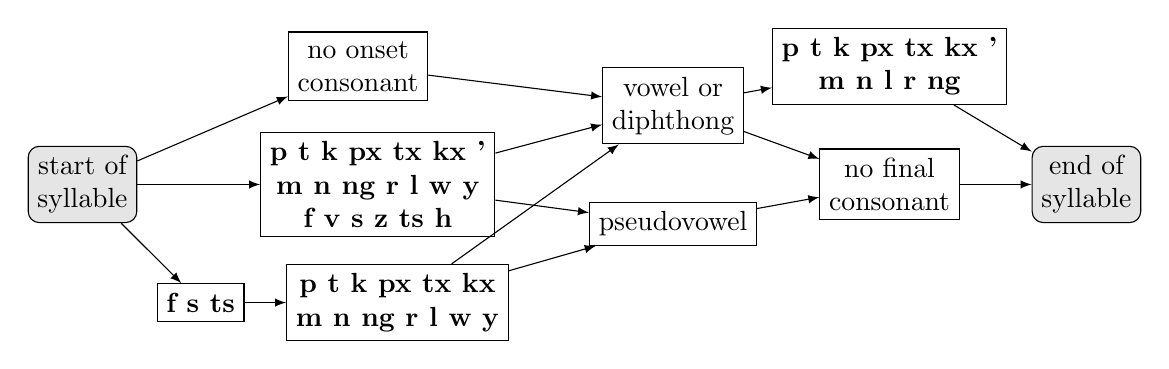
\begin{tikzpicture}[every path/.style={>=latex},every node/.style={draw,rectangle}]
\node[rounded corners,fill=gray!20,align=center] (sos) at (-4,1) {start of\\syllable};
\node[align=center] (zero-onset) at (-0.5,2.5) { no onset\\consonant };
\node[align=center,font=\bfseries] (onset) at (-0.25,1) {p t k px tx kx '\\ m n ng r l w y\\f v s z ts h};
\node[font=\bfseries] (clust-c1) at (-2.5,-0.5) { f s ts };
\node[align=center,font=\bfseries] (clust-c2) at (0,-0.5) {p t k px tx kx\\m n ng r l w y};
\node[align=center] (vowel) at (3.5,2) { vowel or\\diphthong };
\node (pseudovowel) at (3.5,0.5) { pseudovowel };
\node[align=center,font=\bfseries] (final) at (6.25,2.5) {p t k px tx kx ’\\m n l r ng };
\node[align=center] (zero-coda) at (6.25,1) { no final\\consonant };
\node[rounded corners,fill=gray!20,align=center] (eos) at (8.75,1) { end of\\syllable };

\draw[->] (sos) edge (clust-c1);
  \draw[->] (sos) edge (onset);
  \draw[->] (sos) edge (zero-onset);
\draw[->] (clust-c1) edge (clust-c2);
\draw[->] (zero-onset) edge (vowel);
\draw[->] (clust-c2) edge (vowel);
  \draw[->] (clust-c2) edge (pseudovowel);
\draw[->] (onset) edge (vowel);
  \draw[->] (onset) edge (pseudovowel);
\draw[->] (vowel) edge (final);
\draw[->] (final) edge (eos);
\draw[->] (vowel) edge (zero-coda);
\draw[->] (pseudovowel) edge (zero-coda);
\draw[->] (zero-coda) edge (eos);
\end{tikzpicture}
\end{center}

\subsubsection{} Since a syllable may lack a consonant onset or coda,
it is not unusual to see several vowels next to each other in a word.
In that case each vowel is a syllable, \N{muiä} [mu.i.æ], \N{ioang}
[i.o.aŋ].

\subsubsection{} In general, the sequence VCV will be syllabified V.CV
rather than VC.V, so \N{tsenge} is [tsɛ.ŋɛ] not *[tsɛŋ.ɛ].
Onomatopoeia may override this, as in \N{kxang\-ang\-ang} [k'aŋ.aŋ.aŋ],
where the echo effect is desired.

\subsubsection{} There are no long vowels in Forest Na'vi, meaning
identical vowels will not occur next to each other (but see
\horenref{l-and-s:contract}).  Reef Na'vi, due to glottal stop
elision (\horenref{rn:stop-elision}, can have long vowels in several
environments, including by omitting contraction
(\horenref{rn:no-contract}). 

\subsubsection{} Double consonants do not occur in root words, but
may occur at morpheme boundaries, for example in derivations,
\N{tsukkäteng} $<$ \N{tsuk-} $+$ \N{käteng}, or with enclitics
\N{Mo'atta} $<$ \N{Mo'at} $+$ \N{ta} (\horenref{l-and-s:stress:enclisis}).
% https://naviteri.org/2011/03/“receptive-ability”-and-hesitation/comment-page-1/#comment-604

\subsubsection{} As is usual in most Human languages, some
interjections break the rules, such as \N{oìsss}, a sound for anger, or
\N{saa}, a threat cry.


\subsection{Stress Accent}
Every Na'vi word has at least one stress accent, which is not
predictable.  In a very few situations otherwise identical words may
differ only by accent, such as \N{\ACC{tu}te} \E{person}
vs. \N{tu\ACC{te}} \E{woman}.

\subsubsection{} For this word alone, \E{woman}, an accent may be
written in normal Na'vi to indicate the accent, \N{tuté}.
\index{tuté@\textbf{tuté}}

\subsubsection{} Some word creation processes may cause accent shifts
(\horenref{lingop:prefix:ke}, \horenref{lingop:suffix:gender}).

\subsubsection{} All adpositions as well as a few conjunctions and
particles may be enclitic.  They give up their own stress accent and
effectively become part of the word to which they are attached, and
are written so, \N{\ACC{tsa}ne} ($<$ \N{tsaw} $+$ \N{ne}),
\N{ho\ACC{ren}\-ti\-sì} ($<$ \N{ho\ACC{ren}ti} $+$ \N{sì}).
\label{l-and-s:stress:enclisis}\index{enclitics}

\subsubsection{} Though a noun compound is written as a single word,
the individual parts of that compound may each retain their original
accent, as in \N{ti\ACC{re}a\ACC{fya}'o} \E{spirit path}.
\index{compound word!accent}

%\subsubsection{} Word stress is a property of stem words.  No matter
%how many affixes a root word takes, no secondary accents develop.

\subsection{Reef Na'vi} The reef Na'vi dialect has differences in both
consonants and vowels from Forest Na'vi. \index{Reef Na'vi}
\LNWiki{8/1/2022}{http://naviteri.org/2023/01/reef-navi-part-1-phonetics-and-phonology/}

\subsubsection{} An ejective consonant at the start of a syllable—and,
thus, also at the start of a word—is instead pronounced as a voiced
stop in Reef Na'vi.  That is, \N{px tx kx} → [b d g].

\begin{center}
\begin{tabular}{lll}
\N{txon}    & [don] & \E{night} \\
\N{hol\ACC{pxay}} & [hol.ˈbaj] & \E{number} \\
\N{kxitx}   & [git'] & \E{death} \\
\N{skxawng} & [sk'awŋ] (as in Forest Na'vi) & \E{moron}
\end{tabular}
\end{center}

\noindent In general, this change is not spelled out.  That is, Reef
Dialect text will spell \E{night} as \N{txon} but expect the reader to
understand it is pronounced as though \N{don}.  If you wish to
emphasize that the reef dialect is being used, however, it can be
spelled \N{don}.

When a word that ends with an ejective takes a suffix that starts with
a vowel, the pronuncia\-tion of the ejective will adjust to the new
syllable structure.  For example, \N{'awkx} is [ʔawk'], with the
ejective, but \N{'awkxit} is [ˈʔaw.git], with the voiced
pronunciation.
\NTeri{13/1/2023}{http://naviteri.org/2023/01/2653/}

\subsubsection{} When in a cluster with \N{y} the \N{s} and \N{ts}
palatalize.  That is, \N{sy} is pronounced [ʃ] and \N{tsy} is [tʃ].
Due to Na'vi's syllable structure, this can only happen at the start
of a syllable.

\begin{center}
\begin{tabular}{lll}
\N{syaw} & [ʃaw] & \E{call} \\
\N{tsìsyì} & [ˈtsɪ.ʃi] & \E{whisper} (v.in.) \\
\end{tabular}
\end{center}

\noindent This Reef Na'vi sound change is never indicated in spelling.

\subsubsection{} \index{Reef Na'vi!glottal stop elision}\label{rn:stop-elision}
When between two vowels, the glottal stop is normally dropped in Reef
Na'vi.  Both vowels are still distinctly enunciated, even if they are
identical, as in \N{rä'ä} below,

\begin{center}
\begin{tabular}{lll}
\N{fra'u} & \N{frau} & \E{everything} \\
\N{Lo'ak} & \N{Loak} & \E{Lo'ak} (personal name) \\
\N{rä'ä}  & \N{rää} & \E{don't}
\end{tabular}
\end{center}

\noindent This change is also present to a certain degree in Forest
Na'vi, such as with the name \N{Lo'ak} (\horenref{names-with-oa}).

While the glottal stop is retained at the start and end of words, when
affixes are added which then place the stop between vowels the stop
may be dropped.  For example, the phrase for \E{humorous person}
is \N{tute a'ipu} in Forest Na'vi, but \N{tute aipu} in Reef Na'vi, or
the adverb \N{nìaw} rather than Forest Na'vi \N{nì'aw}.
\NTeri{14/1/2023}{http://naviteri.org/2023/01/2653/\#comment-45068}

\subsection{Spoken Alphabet}
Except for \N{tìftang}, the glottal stop, the names of the phonemes
encode information about how the sound is used.  They also have
unusual capitalization when written out: \index{alphabet!spoken}

\begin{center}\small
\begin{tabular}{lll}
\N{tìftang} & \N{Ì} & \N{ReR} \\
\N{A}  & \N{KeK}   & \N{'Rr} \\
\N{AW} & \N{KxeKx} & \N{Sä} \\
\N{AY} & \N{LeL}   & \N{TeT} \\
\N{Ä}  & \N{'Ll}   & \N{TxeTx} \\
\N{E}  & \N{MeM}   & \N{Tsä} \\
\N{EW} & \N{NeN}   & \N{U} \\
\N{EY} & \N{NgeNg} & \N{Vä} \\
\N{Fä} & \N{O}     & \N{Wä} \\
\N{Hä} & \N{PeP}   & \N{Yä} \\
\N{I}  & \N{PxePx} & \N{Zä} \\
\end{tabular}
\end{center}

\subsubsection{} Vowels and diphthongs are simply pronounced and
spelled as themselves.  The pseudo\-vowels take a leading glottal stop,
since they require a consonant onset (\horenref{l-and-s:pseudo-no-null}).

\subsubsection{} The name for consonants which cannot end a syllable
are formed by adding \N{ä}, as in \N{Tsä}.  Those which can end a
syllable use the vowel \N{e} and repeat the consonant at the end of
the name, \N{PeP}.


\section{Lenition}
\noindent Certain grammatical processes cause changes in the first
consonant of a word.  This change is called ``lenition.''  Only eight
consonants undergo lenition.\index{lenition}\label{l-and-s:lenition}
\LanguageLog

\begin{center}
\begin{tabular}{lll}
Consonant & Lenition & Example \\
\N{px, tx, kx} & \N{p, t, k} & \N{\uwave{tx}ep} but \N{mì \uwave{t}ep} \\
\N{p, t, k} & \N{f, s, h} & \N{\uwave{k}elku} but \N{ro \uwave{h}elku} \\
\N{ts} & \N{s} & \N{\uwave{ts}mukan} but \N{ay\uwave{s}mukan} \\
\N{’} & disappears & \N{’eylan} but \N{fpi eylan} \\
\end{tabular}
\end{center}

\noindent In the interlinears, lenition is removed in the
morphological breakdown on the second line (as in
ex.\ref{lenition:ex01} below).

\subsection{Glottal Stop} The glottal stop is not lenited when it is
followed by a pseudovowel (\N{mì 'Rrta} not *\N{mì Rrta}).
\index{glottal stop!lenition}\label{l-and-s:lenition:pseudovowel}
\NTeri{3/28/2012}{https://naviteri.org/2012/03/spring-vocabulary-part-1/}

\subsection{Adpositions} A few adpositions cause lenition when they
precede a word: \N{fpi}, \N{ìlä}, \N{mì}, \N{nuä}, \N{ro}, \N{sko},
\N{sre} (and derived \N{lisre} and \N{pxisre}), \N{wä}. When suffixed
they do not cause lenition in either the word they are attached to or
to the following word.
\index{fpi@\textbf{fpi}!lenition}\index{ilä@\textbf{ìlä}!lenition}
\index{miì@\textbf{mì}!lenition}\index{ro@\textbf{ro}!lenition}
\index{sre@\textbf{sre}!lenition}\index{pxisre@\textbf{pxisre}!lenition}
\index{waä@\textbf{wä}!lenition}\index{nuaä@\textbf{nuä}!lenition}
\index{sko@\textbf{sko}!lenition}
\index{lenition!adpositions}\index{adpositions!lenition}
\NTeri{7/7/2010}{https://naviteri.org/2010/07/thoughts-on-ambiguity/}

\subsection{Number Prefixes} Prefixes which cause lenition are
indicated with a plus sign, rather than the usual dash, as in \N{ay+},
the leniting plural prefix. \index{lenition!number prefixes}

\subsection{Question Prenoun} When used as a prefix, the question
prenoun \N{pe+} causes lenition (\horenref{morph:pre:pe}), as
in \N{pehem} \E{what (action)?} from \N{kem} \E{actition, activity}.

\subsection{Numbers}\index{lenition!numbers}
Suffixed, dependent forms of the numbers are lenited
(\horenref{numbers:dependent}), as in \N{vopey} \E{eleven (8 + 3)},
but \N{pxey} \E{three}.

\subsection{Proper Nouns} Proper nouns still undergo lenition.

\begin{interlin} \label{lenition:ex01}
\glll Oe kelku si mì Helutral. \\
      oe kelku si mì Kelutral \\
     \I{1sg} home do in hometree \\
\trans{I live in hometree}
\end{interlin}

\index{lenition!proper nouns}\NTeri{10/28/2010}{https://naviteri.org/2010/09/getting-to-know-you-part-2/}

\subsection{Reef Na'vi} \index{Reef Na'vi!lenition}
Although the ejectives in Reef Na'vi surface as voiced stops at the
start of a word, the rules of lenition still apply as in Forest Na'vi.
That is, though \N{txon} \E{night} is pronounced as \N{don} in Reef
Na'vi, the lenited form is still \N{ton}.
\LNWiki{8/1/2023}{http://naviteri.org/2023/01/reef-navi-part-1-phonetics-and-phonology/}

\section{Morphophonology}

\subsection{Vowel Contraction} Since identical vowels may not occur
next to each other, a few grammatical processes involve a doubled
vowel reducing to just one.\index{vowel!contraction}\label{l-and-s:contract}

\subsubsection{} The adjective morpheme \N{-a-} disappears when
attached to an \N{a} at the start or end of an adjective, as in
\N{apxa tute} not *\N{apxaa tute}.
\index{-a-@\textbf{-a-}!with \textbf{a} in an adjective}
\index{adjective!contraction}

\subsubsection{} When the dual and trial prefixes leave a sequence of
two \N{e}s, as in \N{me} $+$ \N{'eveng} $>$ *\N{meeveng} (note
lenition), the two vowels contract to just one, \N{meveng}.
\label{l-and-s:phonotactics:nsc} \index{dual!contraction}
\index{trial!contraction}
\LNWiki{20/1/2010}{https://wiki.learnnavi.org/index.php/Canon\%23Extracts_from_various_emails}

\subsubsection{} When the prenoun prefixes end in the same vowel the
following word starts with, they reduce to one, as in \N{tsatan} $<$
\N{tsa-} $+$ \N{atan}, \N{fìlva} $<$ \N{fì-} $+$ \N{ìlva}
(\horenref{morph:prenoun:contraction}).\footnote{The glottal stop is a
consonant, so \N{fì'ìheyu} from \N{fì-} $+$ \N{'ìheyu}.}
\label{l-and-s:phonotactics:precontract}\index{prenoun!contraction}
\LNWiki{18/5/2011}{https://wiki.learnnavi.org/index.php/Canon/2011/April-December\%23Kawtseng.2C_tsapo_and_prefixes}

\subsubsection{} Contraction does not occur for indefinite \N{-o} or
enclitic adpositions.  When two identical vowels occur next to each
other, they are written with a hyphen between them, \N{fya'o-o}
\E{some way,} \N{zekwä-äo} \E{under a finger}.\footnote{Though Forest
Na'vi does not technically have long vowels, the effect of long vowels
occurs in this situation.  Take care to pronounce both \N{ä} in a word
such as \N{zekwä-äo}.}\index{vowel!contraction!inhibited}
% https://wiki.learnnavi.org/index.php/Canon/2010/UltxaAyharyuä#Phonological_Questions

\subsubsection{} In Reef Na'vi vowel contraction is not applied.
Forms such as \N{meeveng} or \N{apxaa} remain, where Forest Na'vi
would simplify the doubled vowels.
\index{Reef Na'vi!vowel contraction inhibited}\label{rn:no-contract}
\NTeri{13/1/2023}{http://naviteri.org/2023/01/2653/}

\subsection{Pseudovowel Contraction} Due to the shape of the aspect
infixes, \N{\INF{er}} and \N{\INF{ol}}, it is possible for the
pseudovowels to occur immediately after their consonantal counterpart,
as in \N{*p\INF{ol}ll\ACC{txe}}.  When this happens in an unstressed
syllable, the pseudovowel disappears, \N{pol\ACC{txe}}.  In a
stressed syllable, the infix disappears, \N{*\ACC{f}\INF{er}\ACC{rr}fen} $>$
\N{\ACC{frr}fen}.  Pseudovowels in monosyllables behave as though
unaccented, \N{vol} from \N{*v\INF{ol}ll}. \index{pseudovowel!contraction}
\LNWiki{23/3/2010}{https://wiki.learnnavi.org/index.php/Canon/2010/March-June\%23Misc_Answers}
\NTeri{19/6/2012}{https://naviteri.org/2012/06/spring-vocabulary-part-3/}

\subsection{Affect Infix Epenthesis} When the positive affect infix
\N{\INF{ei}} is followed by the vowel \N{i}, \N{ì} or a pseudovowel, a
\N{y} is inserted, \N{seiyi} $<$ \N{*s\INF{ei}i}, \N{veykrreiyìn} $<$
\N{*veykrr\INF{ei}ìn}; \N{v\INF{ei}yll} $<$ \N{*veill}.
\label{l-and-s:eiy-epenth}
\NTeri{19/6/2012}{https://naviteri.org/2012/06/spring-vocabulary-part-3/}

\subsubsection{Reef Na'vi} \index{Reef Na'vi!affect infix epenthesis}
The dissimilation of \N{seii} into \N{seiyi} does not occur in Reef
Na'vi.
\NTeri{31/1/2023}{http://naviteri.org/2023/01/2653/}


\subsection{Reef Na'vi Voiced Stop Assimilation} \index{Reef Na'vi!voiced stop assimilation}
In Reef Na'vi, when a word has a cluster of ejectives, such as
in \N{atxkxe} \E{land}, regressive voicing assimilation takes place.
That is, the onset voiced stop (*\N{atxge}) causes the voicing of the
previous coda ejective as well, giving, \N{adge}.
Similarly, \N{ekxtxu} \E{rough} is \N{egdu} in Reef Na'vi.
\LNWiki{8/1/2023}{http://naviteri.org/2023/01/reef-navi-part-1-phonetics-and-phonology/}

\subsection{Nasal Assimilation} In many compounds as well as in some
idioms, final nasals assimilate to the position of the following
word, as in \N{lumpe} as a variant of \N{pelun}.  Such assimilation is
not always written, which may make the etymology of a word clearer, as
in \N{zenke} instead of \N{*zengke}, from \N{zene ke}, or in the several
idioms with the verb \N{tìng} \E{give}, \N{tìng mikyun} being pronounced
\N{tìm mikyun}. \index{nasal assimilation} \label{l-and-s:nasalassim}

\subsection{Vowel Harmony} Na'vi has two instances of optional
regressive vowel harmony in verb infixes.\index{vowel!harmony}

\subsubsection{} The subjunctive future infix, \N{\INF{iyev}}, most
frequently appears as \N{\INF{ìyev}}, with backing of the first vowel.

\subsubsection{}\label{l-and-s:eng}
The vowel of the negative attitude infix, \N{\INF{äng}}, may be raised
if it is immedately followed by the vowel \N{i}, becoming \N{\INF{eng}},

\begin{interlin}
\glll Tsap'alute sengi oe. \\
      tsap'alute s\INF{äng}i oe \\
      apology do\INF{\I{neg.aff}} \I{1sg} \\
\trans{I apologize.}
\end{interlin}

\Ultxa{2/10/2010}{https://wiki.learnnavi.org/index.php/Canon/2010/UltxaAyharyu\%C3\%A4\%23.C3.A4ng.2Feng}

\subsection{Elision} In rapid speech final \N{-e} is frequently elided
when the following word starts in a vowel.  \Npawl{Kìyevam$\not$e
ult$\not$e Eywa ngahu}.  This is not indicated in writing.\index{elision}
When the final \N{-e} is in a monosyllable (\N{ke, sre}), or when it is
stressed (\N{tuté}), it is not elided.
\LNForum{25/10/2022}{https://forum.learnnavi.org/language-updates/a-collection-of-questions-answered/}

\subsubsection{} The vowel \N{ì} in \N{mì}, \N{sì} and the adverb
prefix \N{nì-} drops before the plural prefix \N{ay+}, though there is
no change in writing.  So, \N{nìayfo} \E{like them} is pronounced as
\N{nayfo}. \label{l-and-s:elision-i}
\index{miì@\textbf{mì}!elision with plural}
\index{siì@\textbf{sì}!elision with plural}
\index{niì-@\textbf{nì-}!elision with plural}
\NTeri{1/7/2010}{https://naviteri.org/2010/07/thoughts-on-ambiguity/}

\subsubsection{} The vowel in \N{nì-} will usually elide before a
stressed \N{e}, as in \N{nì-} + \N{etrìp} > \N{netrìp}. If the \N{e}
is unstressed, it will usually, though not always, elide, \N{nì-} +
\N{eyawr} > \N{nìyawr}. One exception: \N{nìean} instead of the
expected \N{*nìan}.
\index{niì-@\textbf{nì-}!elision before e}
\LNForum{9/8/2017}{https://forum.learnnavi.org/language-updates/if-ni-will-attached-at-e/}

\subsection{Other Phonetic Processes}

\subsubsection{Names with -o'a-} \label{names-with-oa}
In colloquial speech names containing the sequence \N{o'a} may
eliminate the glottal stop, such
as \N{Mo'at} \textasciitilde{} \N{Moat} 
and \N{Lo'ak} \textasciitilde \N{Loak}.
\NTeri{1/3/2017}{https://naviteri.org/2017/02/ayioang-amip-si-ayu-alahe-new-animals-and-other-things/\#comment-26401}


\section{Orthographic Conventions}
\noindent Na'vi in general follows the spelling, punctuation and
capitalization habits of English, but there are a few differences.

\subsection{Proper Names} When taking lexical prefixes
(\horenref{lingop:affixes}), proper names retain their original
capitalization, as in \N{lì'fya le\uwave{Na'vi}}.

\subsection{Quotation} Direct quotes are not punctuated with quotation
marks in Na'vi.  Instead it relies on the quotation particles
\N{san\dots sìk} (see \horenref{syn:direct-quote}).
\index{quotation!punctuation}

\subsection{Etymological Spelling} In addition to the occasional
spelling of nasals to reflect etymo\-logy (\horenref{l-and-s:nasalassim}),
there are a few grammatical processes which result in spelling that
reflects the grammar more than the pronunciation.

\subsubsection{} The first person pronoun root \N{oe}, though
pronounced \N{we} when taking a suffix, retains the original spelling
(\horenref{morph:pron:oe-we}).

\subsubsection{} Before words starting with \N{y} the plural prefix
\N{ay+} is unchanged, \N{ayyerik}.
\LNWiki{18/4/2010}{https://wiki.learnnavi.org/index.php/Canon/2010/March-June\%23ay.2Byerik}

\subsection{Attributive Phrase Hyphenation} Certain short attributive
phrases are written with hy\-phens joining the elements.

\subsubsection{} Attributive phrases of color using \N{na} \E{like}
are hyphenated, \N{fìsyulang aean-na-ta'leng} \E{this skin-blue
flower} (\horenref{syn:attr:na}).

\subsubsection{} Participles of \N{si} construction verbs are also
hyphenated, \N{srung-susia tute} \E{a helping person}
(\horenref{syn:participle:si-const}).

